\newpage{\pagestyle{empty}\cleardoublepage}
\newpage{\pagestyle{empty}\cleardoublepage}
\newpage
\vspace*{\fill}
    \begin{center}
      \thispagestyle{empty} \vspace*{0cm} \textbf{\huge
Introducci\'{o}n}
    \end{center}
    \vspace*{\fill}
\newpage{\pagestyle{empty}\cleardoublepage}
\chapter{Visi\'{o}n de la aplicaci\'{o}n}
\section{Descripci\'{o}n general}


Se desea desarrollar una aplicaci\'{o}n para el sector de la compraventa y alquiler de viviendas, la cual permit\'{a} un acceso r\'{a}pido y p\'{u}blico del listado de anuncios que se hayan publicado. \\

La aplicaci\'{o} deber\'{a} permitir el listado paginado de los anuncios del sistema, as\'{i} como una serie de par\'{a}metros o filtros para personalizar b\'{u}squedas. Del mismo modo, se requerir\'{a} un buscador global en la p\'{a}gina principal que ayude a los usuarios a localizar de forma sencilla y cercana al lenguaje natural un conjunto de anuncios.\\

Para acceder a m\'{a}s funcionalidades, el sistema deber\'{a} permitir que un usuario pueda registrarse e identificarse en el sistema.\\

El sistema debe permitir tambi\'{e}n la gesti\'{o}n de anuncios a los usuarios registrados que los hayan publicado (anunciantes), incluyendo creaci\'{o}n, edici\'{o}n y eliminaci\'{o}n de \'{e}stos.\\

A partir de los anuncios consultados, el usuario podr\'{a} a\~{n}adir comentarios y consultar los existentes, as\'{i} como valorar los propios anuncios de forma sencilla.\\

Para que los usuarios se sientan c\'{o}modos creando los anuncios, se les proporcionar\'{a} una lista de Operaciones y tipos de viviendas asociadas a los anuncios. Tambi\'{e}n se les facilitar\'{a} la selecci\'{o}n de la comunidad aut\'{o}noma, provincia y municipio. La gesti\'{o}n de im\'{a}genes en los anuncios permitir\'{a} al usuario subir varias a la vez, as\'{i} como sustitu\'{i}rlas de manera sencilla.\\

Sobre un anuncio, un usuario registrado interesado podr\'{a} realizar una petici\'{o}n que aparecer\'{a} al anunciante en su zona adecuada para gestionarla, pudiendo aceptarla (rechazando todas las dem\'{a}s asociadas a este anuncio) o rechazarla. Aquel anuncio que estuviera aceptado no deber\'{i}a aparecer en los resultados de b\'{u}squeda. \\ 

Los usuarios registrados podr\'{a}n denunciar a otros usuarios que hayan llevado mal comportamiento en el sistema, peticiones sobre los propios anuncios que crean inadecuadas, anuncios con contenido ofensivo o comentarios no adecuados para la web.

Para todo este sistema se exigir\'{a} tambi\'{e}n la existencia de un rol administrador, el cual permitir\'{a} acceder a una zona especial y reservada conocida como 'dashboard' y en la que se pueda gestionar al completo los usuarios, anuncios, denuncias, tipos de operaciones y tipos de viviendas.

\section{Descripci\'{o}n Detallada}
\subsection{P\'{a}gina Principal}


El usuario visitante podr\'{a} realizar una b\'{u}squeda globalmente en el sistema a trav\'{e}s de un buscador global, as\'{i} como ver de forma ordenada y paginada el listado global de anuncios, en lo posible filtrado seg\'{u}n el tipo de anuncio (en principio compraventa o alquiler) y su tipo de vivienda (en principio casa o piso). Al usuario logado en el sistema se le permitir\'{a} acceder a su perfil desde el navegador principal. Al Administrador, adem\'{a}s, se le proporcionar\'{a} una v\'{i}a de acceso a la zona de gesti\'{o}n.\\

\begin{figure}[h!]
\centering
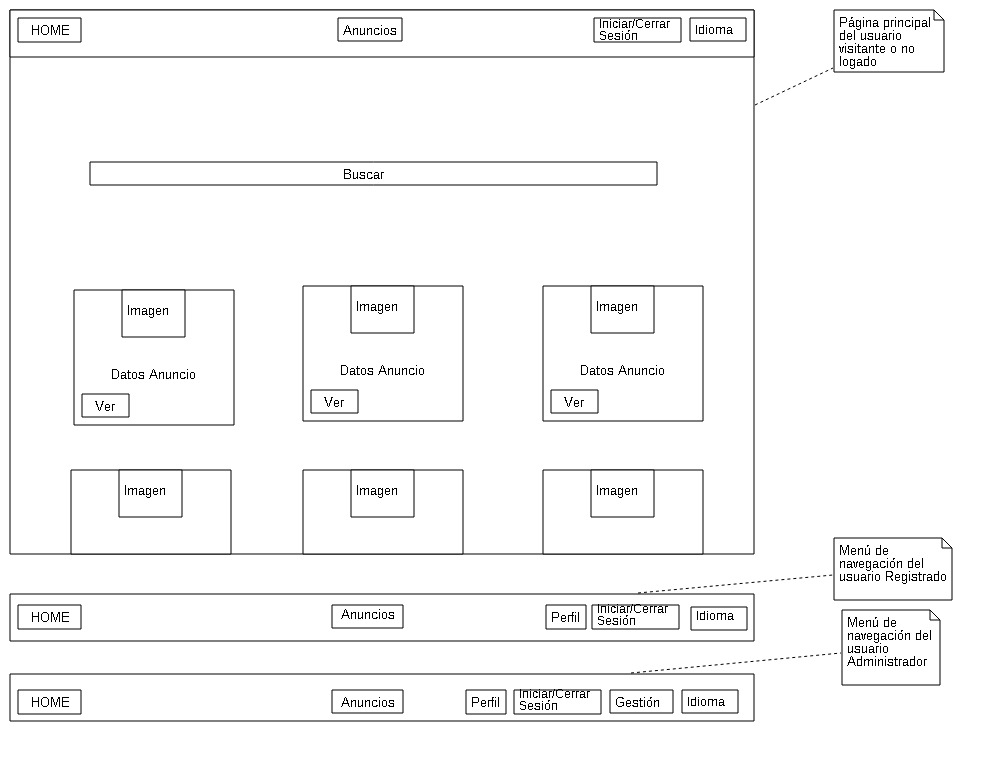
\includegraphics[width=.8\textwidth]{Img/VisionAplicacion/vision_1.jpg}
\end{figure}

Bajo el buscador global aparecer\'{a}n 9 tarjetas adecuadamente situadas con un resumen visual de los \'{u}ltimos 9 anuncios publicados en el sistema, como se plantea en la imagen siguiente:



A trav\'{e}s de estos resultados mostrados se podr\'{a} acceder a los detalles del anuncio en cuesti\'{o}n.\\

En el bot\'{o}n primero del men\'{u} de navegaci\'{o}n superior se mostrar\'{a} alg\'{u}n tipo de imagen o mensaje intuitivo, de forma que el usuario entienda que al hacer click se volver\'{a} a la p\'{a}gina principal.

\subsection{Registro y Login}

Para iniciar sesi\'{o}n en el sistema har\'{a} falta que el usuario est\'{e} registrado. En caso de no estarlo, en la misma secci\'{o}n de acceso se deber\'{a} facilitar al usuario un formulario de inscripci\'{o}n, m\'{i}nimamente con los datos nombre, apellidos, email, tel\'{e}fono, usuario (o username)y contrase\~{n}a. Todos estos datos ser\'{a}n obligatorios. 


\begin{figure}[h!]
\centering
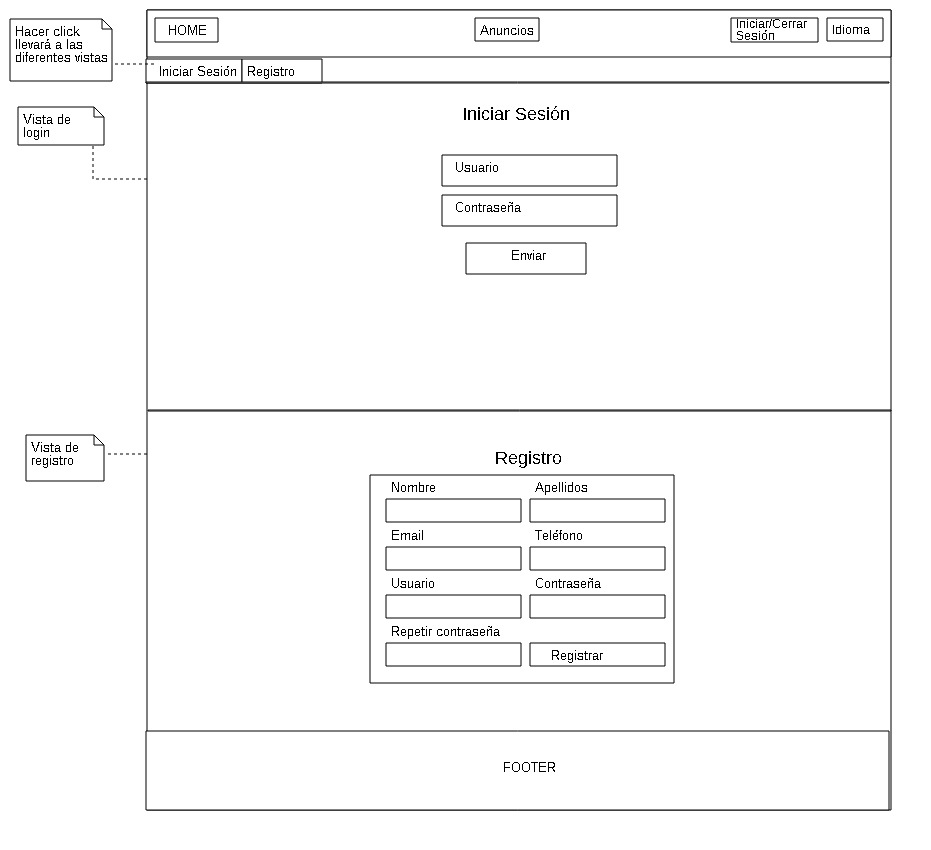
\includegraphics[width=.9\textwidth]{Img/VisionAplicacion/vision_2.jpg}
\end{figure}


\subsection{Listado de anuncios}
El usuario invitado (as\'{i} como registrado o administrador) podr\'{a} listar el conjunto total de anuncios paginados correctamente y con la posibilidad de filtrar por tipo de operaci\'{o}n (como alquiler o compra) y tipo de vivienda (piso o casa). No se deber\'{a}n cargar muchos resultados por p\'{a}gina. De los anuncios se requiere mostrar una miniatura de alguna de sus im\'{a}genes, en caso de tener, un t\'{i}tulo asociado al tipo de vivienda y su zona, su precio, habitaciones, metros cuadrados y localizaci\'{o}n. Tambi\'{e}n su descripci\'{o}n limitada a unas pocas palabras y cu\'{a}ndo se public\'{o}. A trav\'{e}s de estos resultados mostrados se podr\'{a} acceder a los detalles del anuncio en cuesti\'{o}n.

Esta misma vista ser\'{a} utilizada para listar los anuncios de un usuario en particular.


\begin{figure}[h!]
\centering
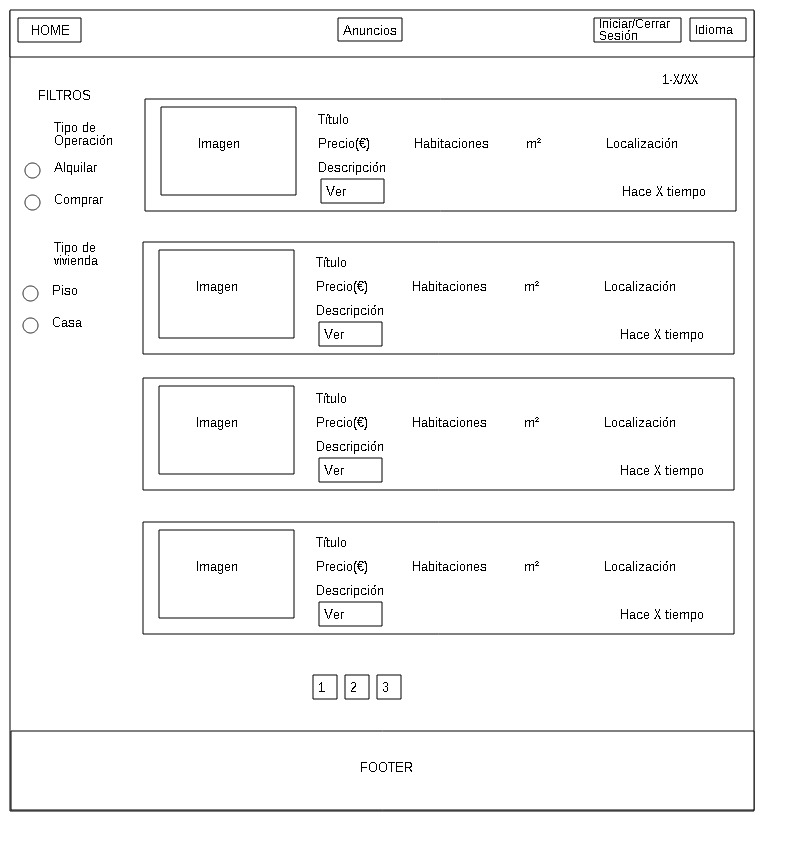
\includegraphics[width=.8\textwidth]{Img/VisionAplicacion/vision_3.jpg}
\end{figure}

En caso de haber utilizado el buscador global y haber pulsado intro al escribir se mostrar\'{a} una p\'{a}gina con contenido similar al listado de anuncios, pero sin posibilidad de filtrar. El aspecto de las tarjetas mostradas ser\'{a} el mismo que las listadas en la p\'{a}gina principal. Se paginar\'{a} este resultado.

\begin{figure}[h!]
\centering
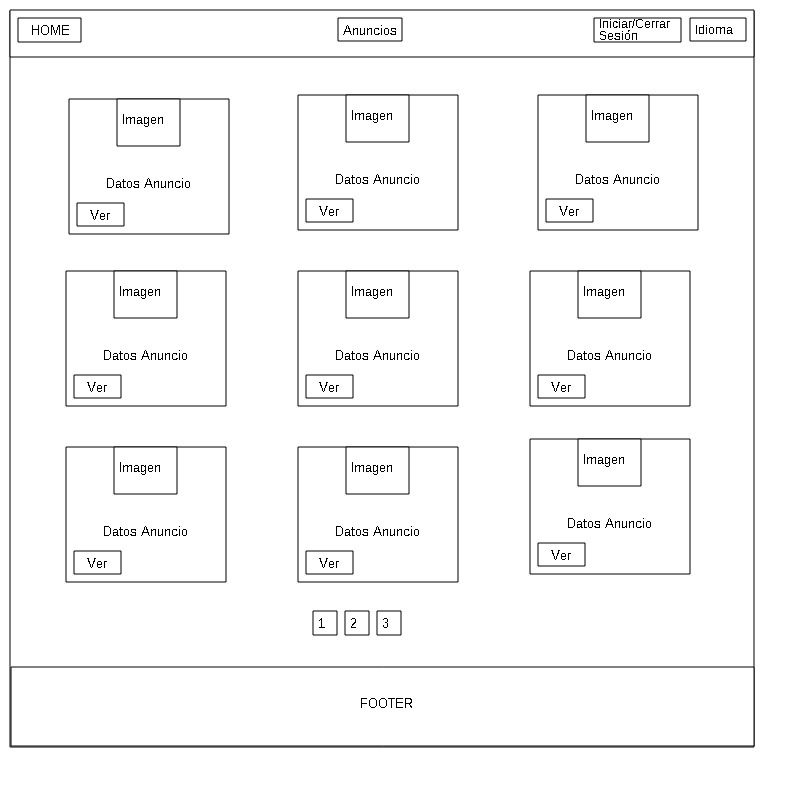
\includegraphics[width=1\textwidth]{Img/VisionAplicacion/vision_10.jpg}
\end{figure}


\subsection{Perfil de Usuario}
A trav\'{e}s del men\'{u} principal, cada usuario podr\'{a} consultar su propio perfil, donde podr\'{a} en contrar un formulario con sus datos para editarlos, menos correo electr\'{o}nico y nombre de usuario.\\

Tambi\'{e}n existir\'{a} un panel de informaci\'{o}n con la cantidad de anuncios publicados por el usuario (y a trav\'{e}s del cual se podr\'{a} llegar al listado mostrado en el punto anterior) y comentarios.\\

Paginando una tarjeta junto a los datos del perfil del usuario, se mostrar\'{a} una peque\~{n}a tabla con el listado de solicitudes que el usuario haya recibido en sus anuncios. Se mostrar\'{a} el usuario asociado a la solicitud, contacto y el contenido escrito por el mismo para ponerse en contacto. Se le facilitar\'{a} al usuario registrado la posibilidad de denunciar dicha solicitud, aceptarla y rechazarla.

\begin{figure}[h!]
\centering
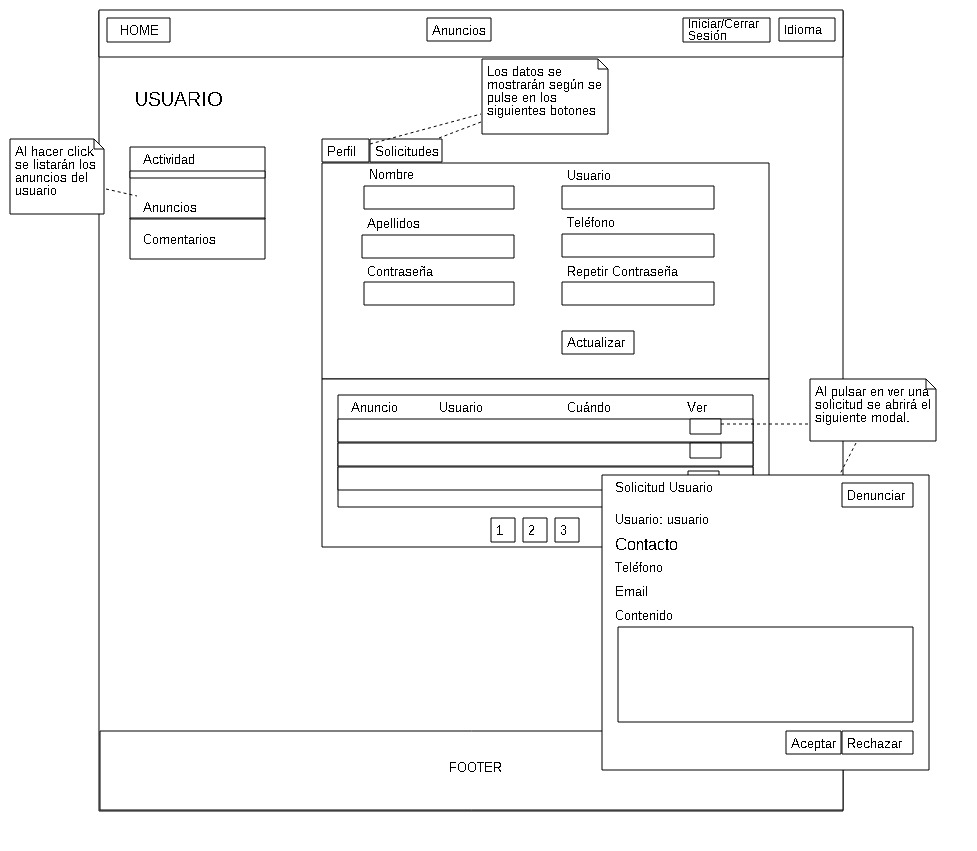
\includegraphics[width=1\textwidth]{Img/VisionAplicacion/vision_4.jpg}
\end{figure}

Por otro lado, si se consultara al usuario asociado a la solicitud o cualquier otro usuario, se mostrar\'{i}a la siguiente vista, donde s\'{o}lamente se muestran sus datos, sin posibilidad de editar. El usuario administrador dispondr\'{a} de dos botones extra para bloquear o eliminar al usuario.\\

\begin{figure}[h!]
\centering
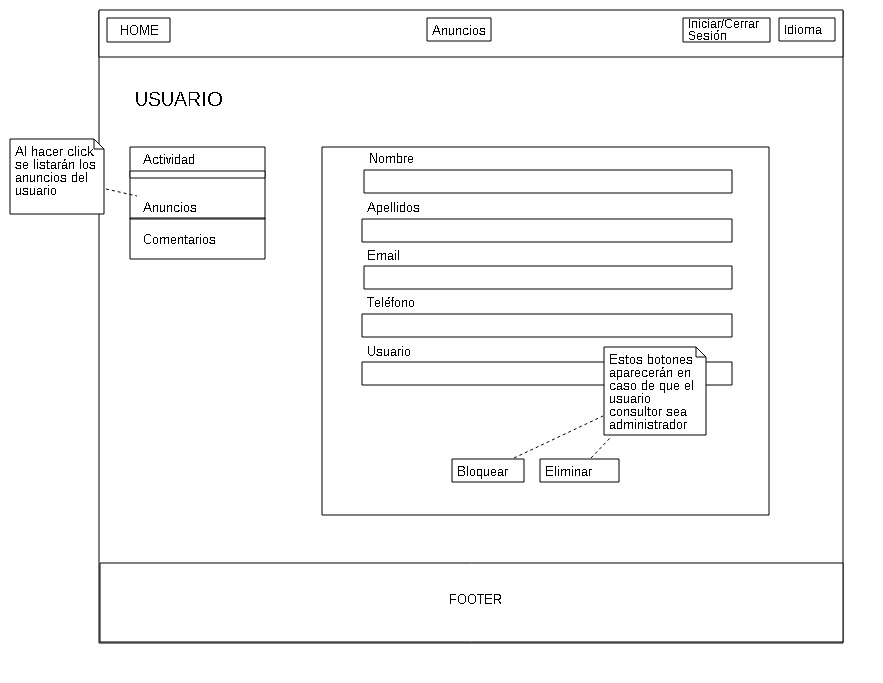
\includegraphics[width=1\textwidth]{Img/VisionAplicacion/vision_5.jpg}
\end{figure}

\subsection{Anuncios}

Al consultar un anuncio desde cualquier vista se observar\'{a}n todos los detalles asociados al mismo: 
tipo de vivienda, tipo de operaci\'{o}n, precio n\'{u}mero de habitaciones, metros cuadrados, n\'{u}mero de ba\~{n}os, descripci\'{o}n, comunidad aut\'{o}noma, provinciay localidad.\\

Tambi\'{e}n se mostrar\'{a} una galer\'{i}a de fotos, donde se permitir\'{a} ampliar las im\'{a}genes haciendo click en ellas.\\

Debajo de \'{e}stas aparecer\'{a} un peque\'~{n}o formulario para crear un comentario, en caso de que el usuario haya iniciado sesi\'{o}n, seguido de un listado de comentarios previamente existentes que se podr\'{a} consultar sin sesi\'{o}n activa. En caso de estar logado en el sistema se podr\'{a} denunciar un comentario si se cree conveniente.\\

\begin{figure}[h!]
\centering
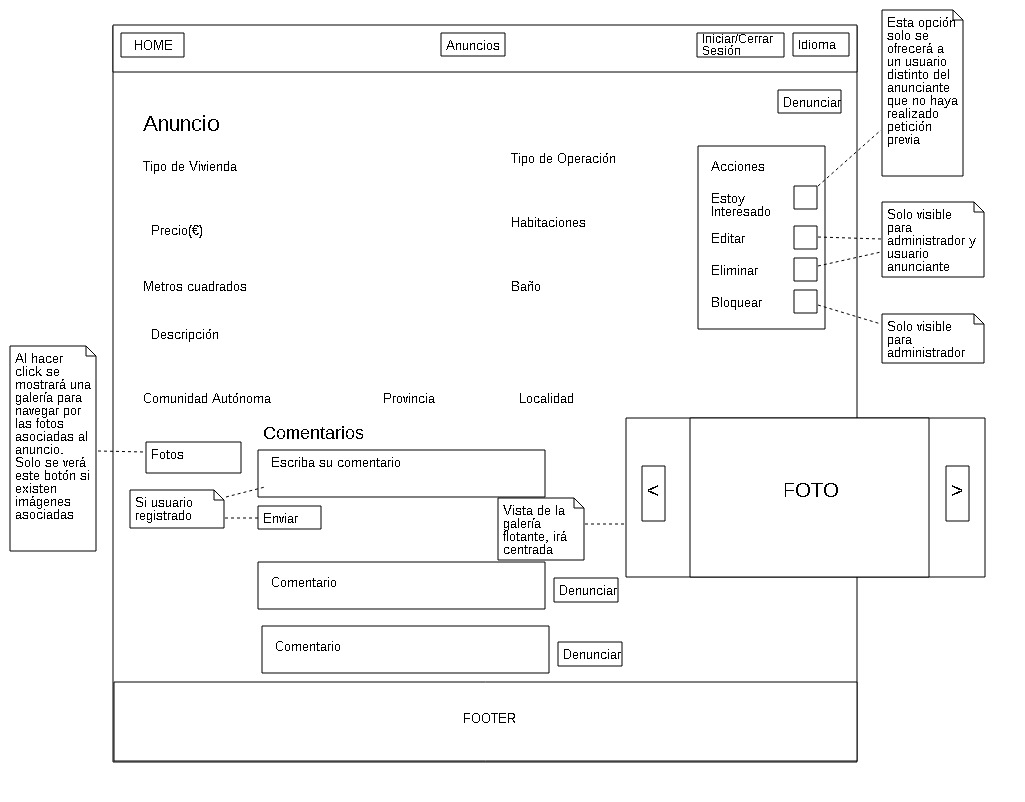
\includegraphics[width=1\textwidth]{Img/VisionAplicacion/vision_6.jpg}
\end{figure}

A la derecha de los datos del anuncio se ver\'{a} un peque\~{n}o panel que muestre las acciones disponibles sobre el anuncio, como realizar una petici\'{o}n (en caso de no ser el propio anunciante o existir una petici\'{o}n previa del usuario sobre ese mismo anuncio), edici\'{o}n y eliminaci\'{o}n (si administrador o usuario anunciante) o bloqueo del anuncio (si usuario administrador). \\

Encima de este panel se ofrecer\'{a} un bot\'{o}n para denunciar el anuncio.




\subsection{Creaci\'{o}n de anuncios}



Los usuarios que quieran publicar un anuncio deber\'{a}n registrarse y logarse en el sistema. 
En el alta del anuncio el usuario decidir\'{a} si quiere ofrecer una venta o alquiler, su precio, metros cuadrados, descripci\'{o}n y aportar fotos. \\

Del mismo modo, se proveer\'{a} a los usuarios de la posibilidad de modificar y retirar sus anuncios. 


\begin{figure}[h!]
\centering
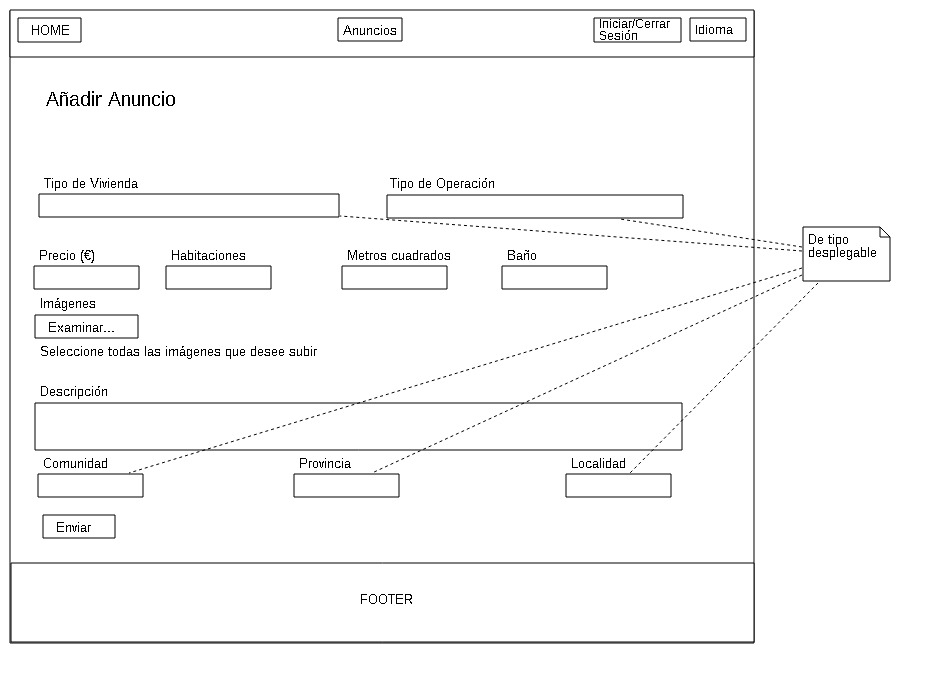
\includegraphics[width=1\textwidth]{Img/VisionAplicacion/vision_7.jpg}
\end{figure}


\subsection{Administrar Usuarios}
Del usuario administrador se espera que se pueda realizar las mismas funciones que un usuario registrado, aparte de sus tareas de administraci\'{o}n, como puedan ser la gesti\'{o}n de usuarios, anuncios y comentarios, de forma que si alg\'{u}n comentario o anuncio fuera ofensivo, \'{e}ste lo borrar\'{i}a y bloquear\'{i}a al usuario, o si existiera alguna denuncia asociada a alguno de estos y fuera debidamente revisada y verificada, se podr\'{i}a aceptar y bloquear autom\'{a}ticamente o, por el contrario, rechazar.

\begin{figure}[h!]
\centering
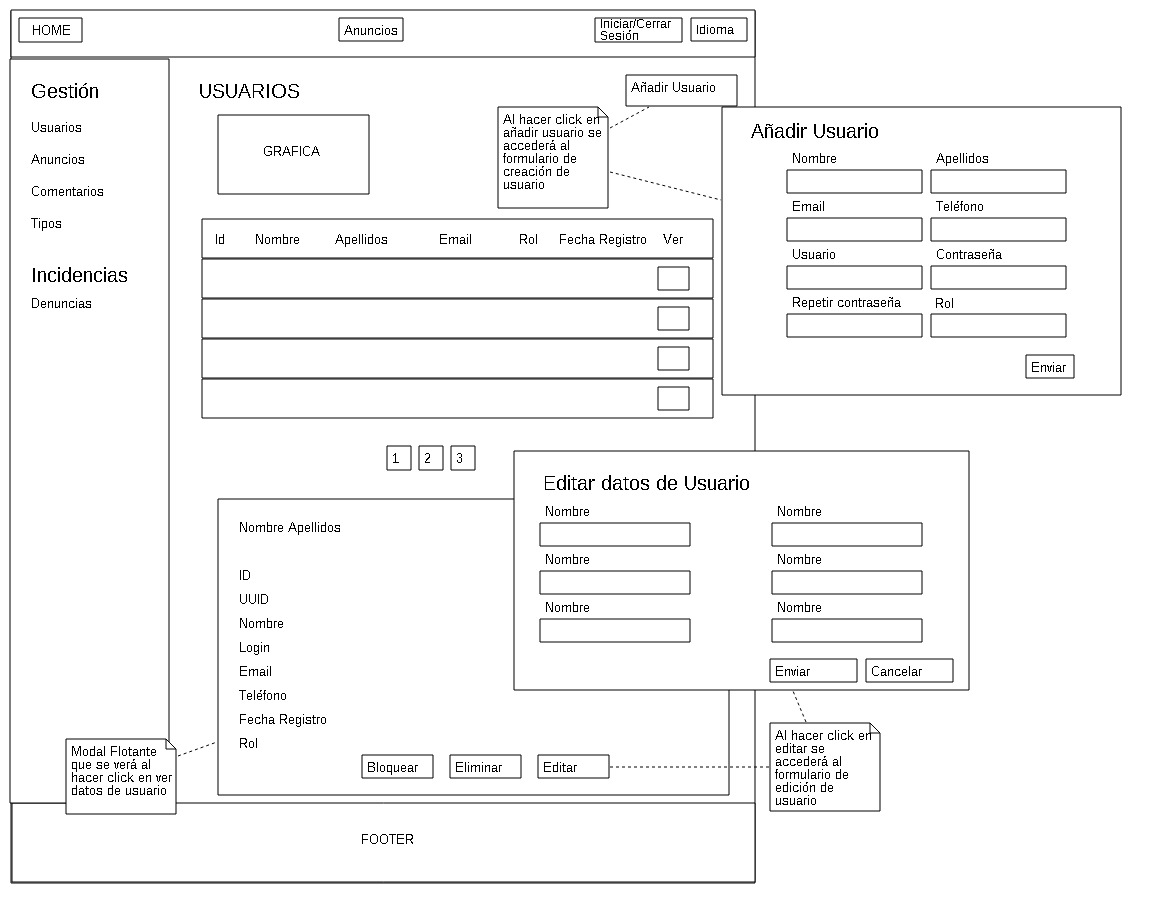
\includegraphics[width=1\textwidth]{Img/VisionAplicacion/vision_8.jpg}
\end{figure}



Primeramente, el usuario administrador ver\'{a} en su zona de administraci\'{o}n o 'dashboard' un listado de usuarios, un gr\'{a}fico con el n\'{u}mero de registros en el sistema filtrado por mes y a\~{n}o y algunos de los datos de los usuarios en una tabla debidamente paginada: id, nombre, apellidos, email, rol, fecha de registro y un bot\'{o}n que permita consultar el resto de datos asociados al usuario y acceder a m\'{a}s funcionalidades, como editar, eliminar o bloquear paginada correctamente.





\subsection{Administrar Anuncios}
El usuario administrador podr\'{a} acceder desde su panel lateral en la zona de administraci\'{o}n a la gesti\'{o}n de los anuncios, en donde encontrar\'{a} una tabla con el id, uuid, precio, fecha registro y un bot\'{o}n que env\'{i}e a la consulta del anuncio seleccionado. Por supuesto, esta tabla estar\'{a} debidamente paginada.



\begin{figure}[h!]
\centering
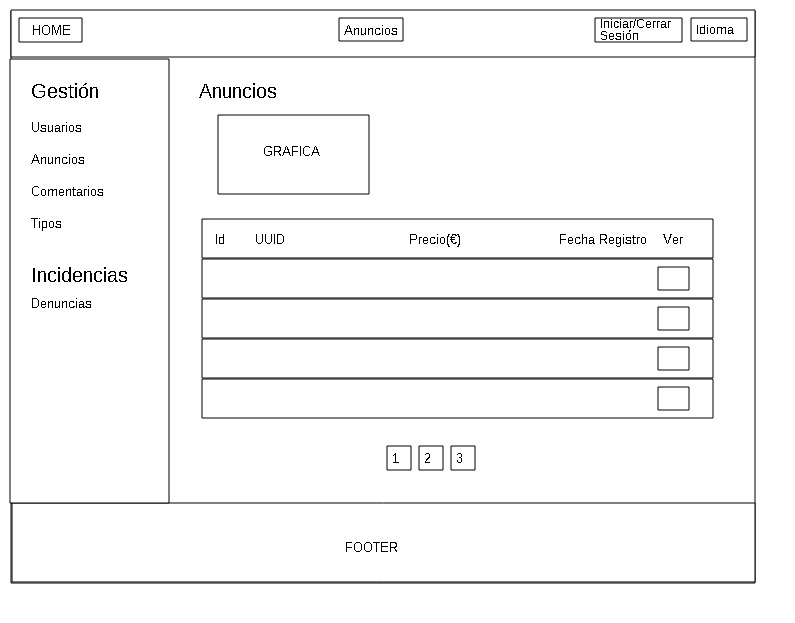
\includegraphics[width=1\textwidth]{Img/VisionAplicacion/vision_9.jpg}
\end{figure}

\subsection{Administrar Comentarios}
\subsection{Administrar Tipos}
\subsection{Administrar Denuncias}

